\section*{Phụ Lục: Minh Họa Kiểm Chứng Định Dạng và Thực Nghiệm Trực Quan}
\addcontentsline{toc}{section}{Phụ lục: Minh họa kiểm chứng định dạng và thực nghiệm trực quan}

Phần phụ lục bổ sung các bằng chứng trực quan nhằm xác minh tính hợp lệ của dữ liệu đầu ra theo quy định hiện hành. Trước hết, các hình từ Hình~\ref{fig:ppocr_ch} đến Hình~\ref{fig:csv_preview} kiểm chứng trực tiếp định dạng hộp tọa độ bốn điểm chuẩn PPOCRLabel trên trang Hán Nôm và trang Quốc ngữ, khả năng mở tệp bảng tính \texttt{.xlsx} với đầy đủ màu chữ ngữ nghĩa không lỗi font, cũng như tính nhất quán năm cột của tệp \texttt{.csv}. Tiếp theo, Hình~\ref{fig:line_boxes} và Hình~\ref{fig:parallel_align} minh họa kết quả tách dòng trên giấy ố vàng và kết quả chiếu ranh giới câu song ngữ giữa hai hệ chữ viết đọc ngược chiều.

\subsection*{A. Kiểm chứng chuẩn định dạng PPOCRLabel, trang tính \texttt{.xlsx} và \texttt{.csv}}

\begin{figure}[H]
    \centering
    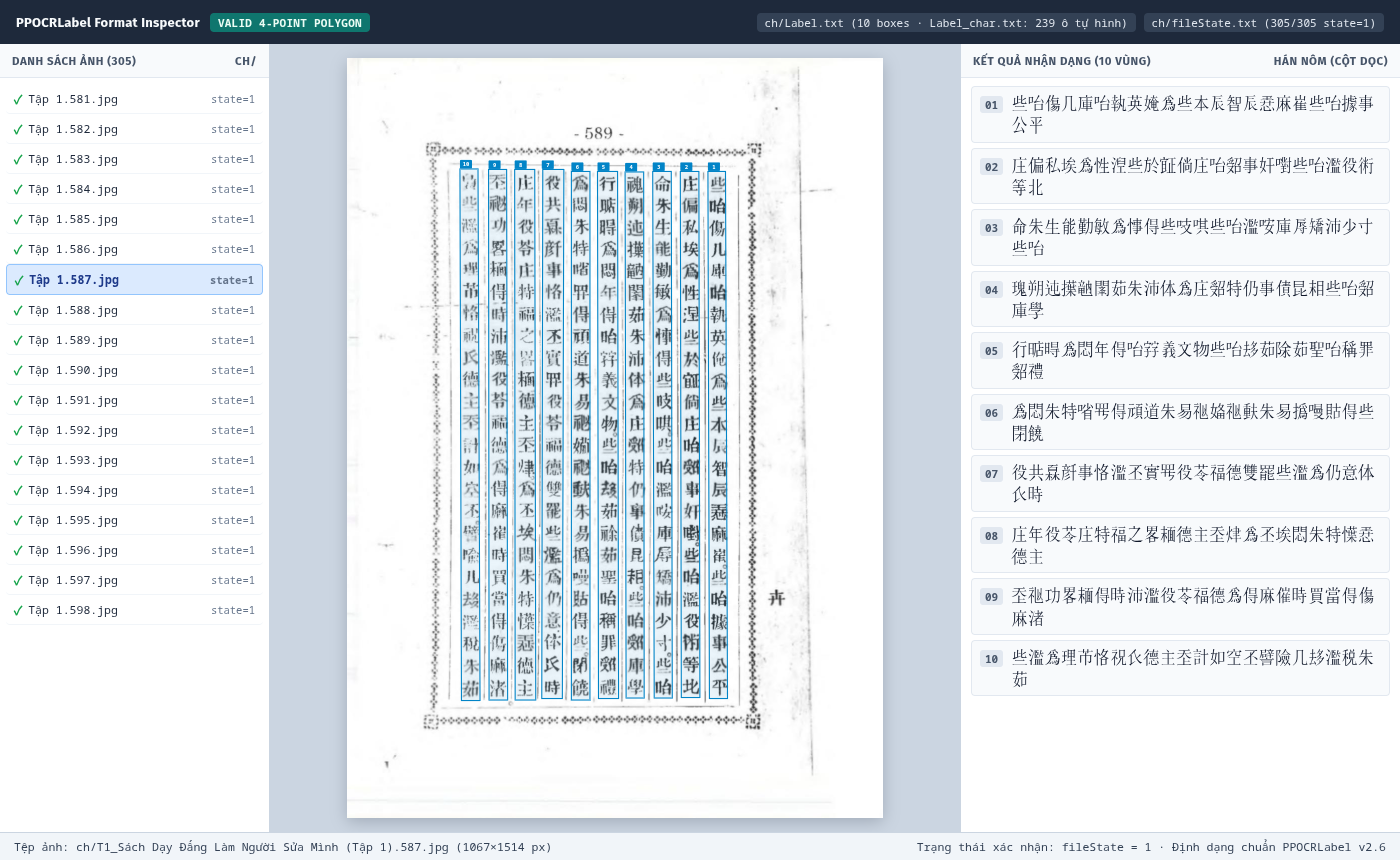
\includegraphics[width=\linewidth]{images/appendix_ppocr_ch.png}
    \caption{Kiểm chứng trực quan định dạng PPOCRLabel trên trang Hán Nôm mẫu (Tập 1, trang $587$): toàn bộ $10$ cột chữ dọc khớp khung đa giác $4$ điểm, trạng thái xác nhận hợp lệ trên $305/305$ trang cùng $239$ khung tự hình đơn}
    \label{fig:ppocr_ch}
\end{figure}

\begin{figure}[H]
    \centering
    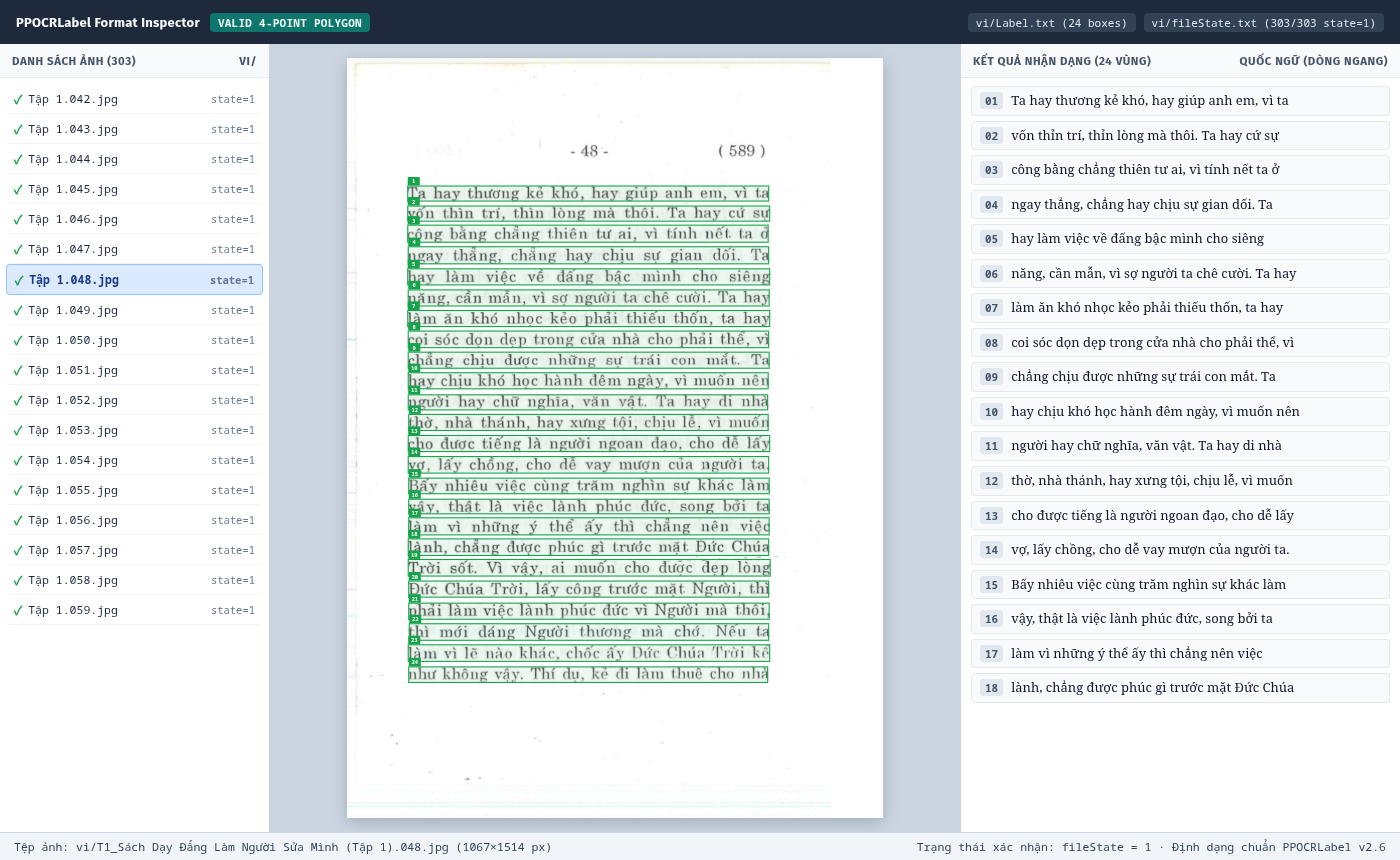
\includegraphics[width=\linewidth]{images/appendix_ppocr_vi.png}
    \caption{Kiểm chứng trực quan định dạng PPOCRLabel trên trang Quốc ngữ mẫu (Tập 1, trang $048$): toàn bộ $24$ dòng thân trang khớp khung đa giác $4$ điểm, dòng tiêu đề số trang đã được tách bỏ, trạng thái xác nhận hợp lệ trên $303/303$ trang}
    \label{fig:ppocr_vi}
\end{figure}

\begin{figure}[H]
    \centering
    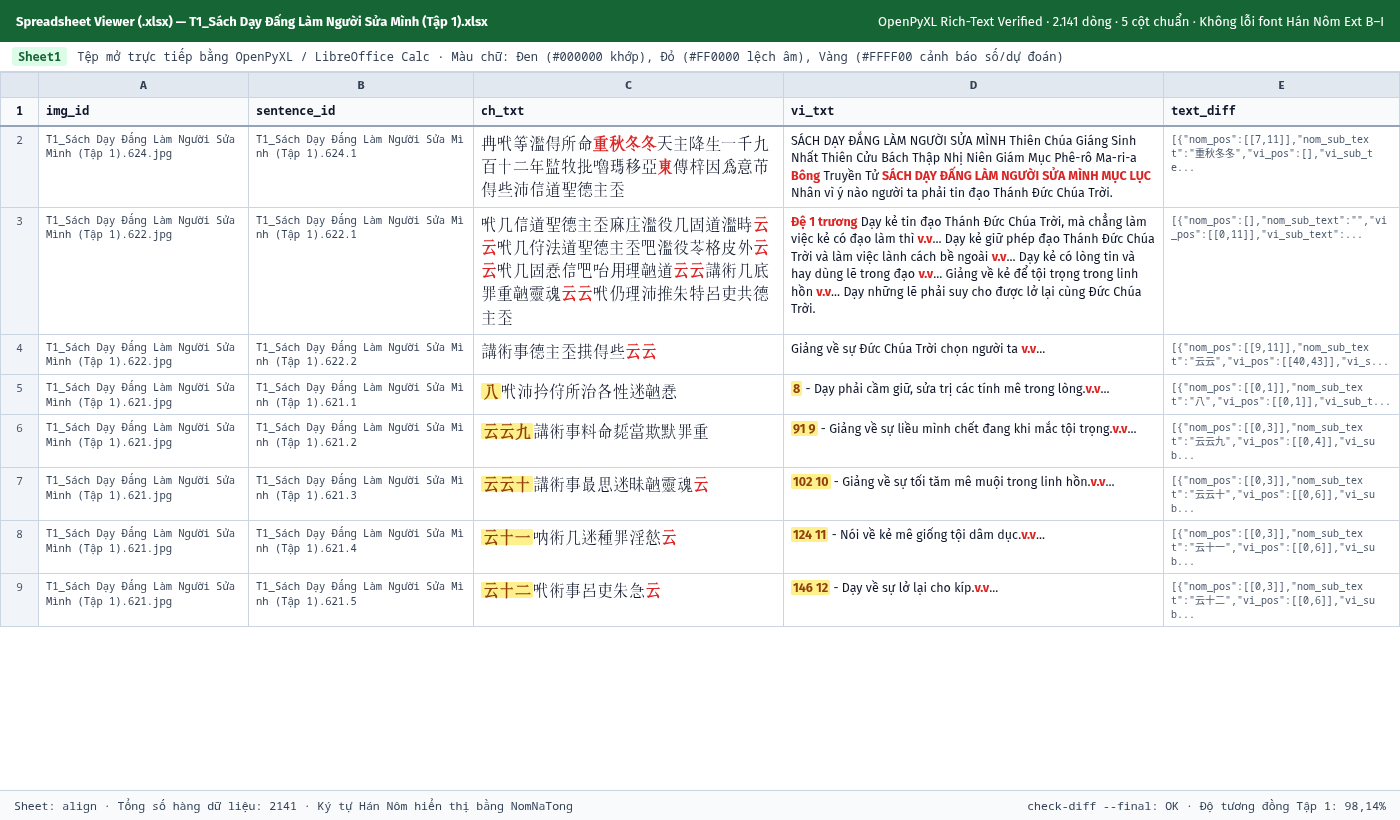
\includegraphics[width=\linewidth]{images/appendix_xlsx_preview.png}
    \caption{Kiểm chứng trang tính \texttt{.xlsx} của Tập 1 (hiển thị dữ liệu rich-text đọc trực tiếp từ tệp nộp): các tự hình Hán Nôm mở rộng hiển thị rõ nét không lỗi font và giữ đúng ba màu ngữ nghĩa (đen: khớp âm, đỏ: bất tương đồng, vàng: cảnh báo số học)}
    \label{fig:xlsx_preview}
\end{figure}

\begin{figure}[H]
    \centering
    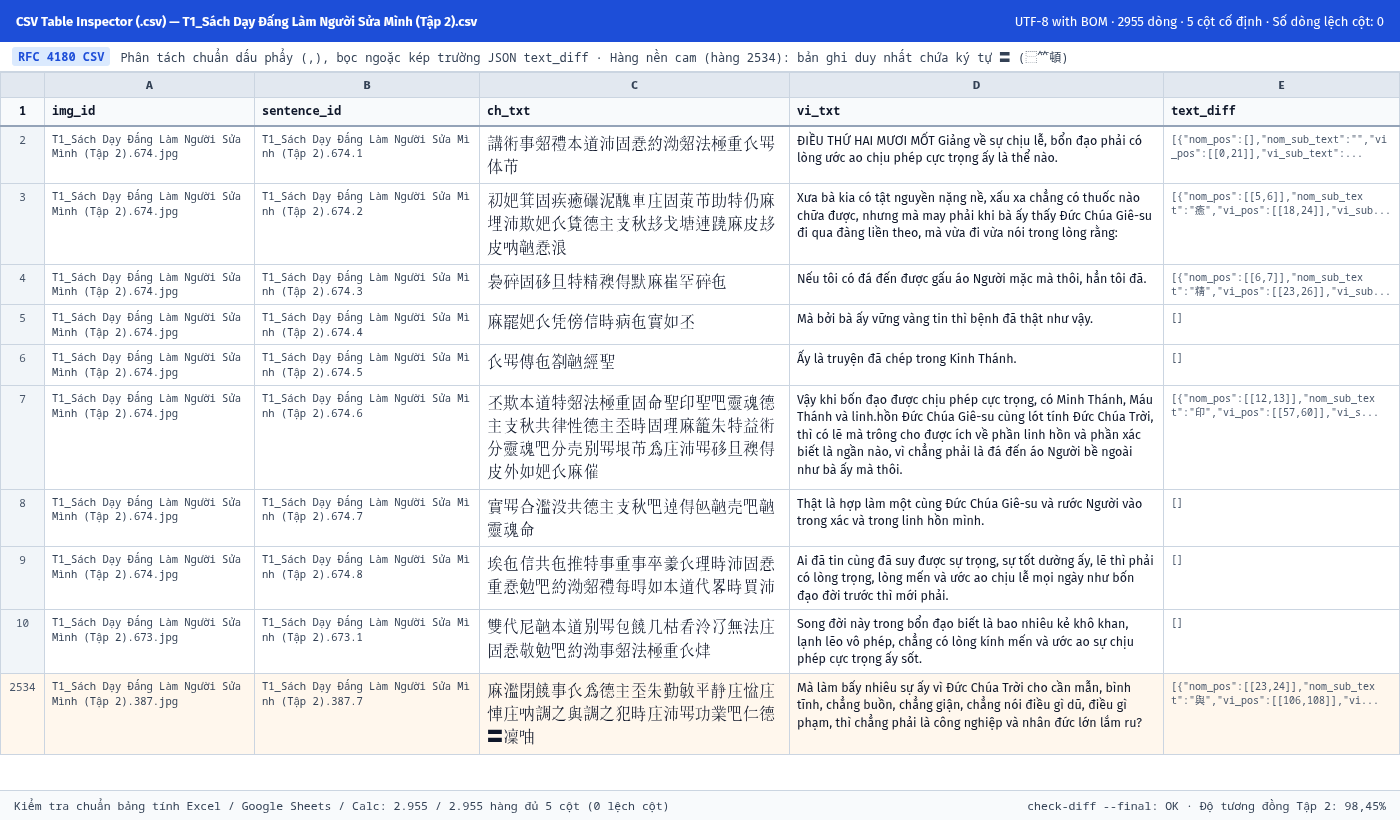
\includegraphics[width=\linewidth]{images/appendix_csv_preview.png}
    \caption{Kiểm chứng trang tính \texttt{.csv} của Tập 2 (mã hóa UTF-8 có BOM, $2.955$ dòng đủ đúng $5$ cột, $0$ dòng lệch cột): hàng nổi bật cuối cùng minh họa bản ghi duy nhất trên hai tập chứa ký tự đại diện ngoài chuẩn Unicode \nom{〓} (\ids{⿱}\nom{𥫗頓}, âm \textit{lớn})}
    \label{fig:csv_preview}
\end{figure}

\subsection*{B. Minh họa thực nghiệm tách dòng và chiếu ranh giới câu song ngữ}

\begin{figure}[H]
    \centering
    \begin{subfigure}[t]{0.48\linewidth}
        \centering
        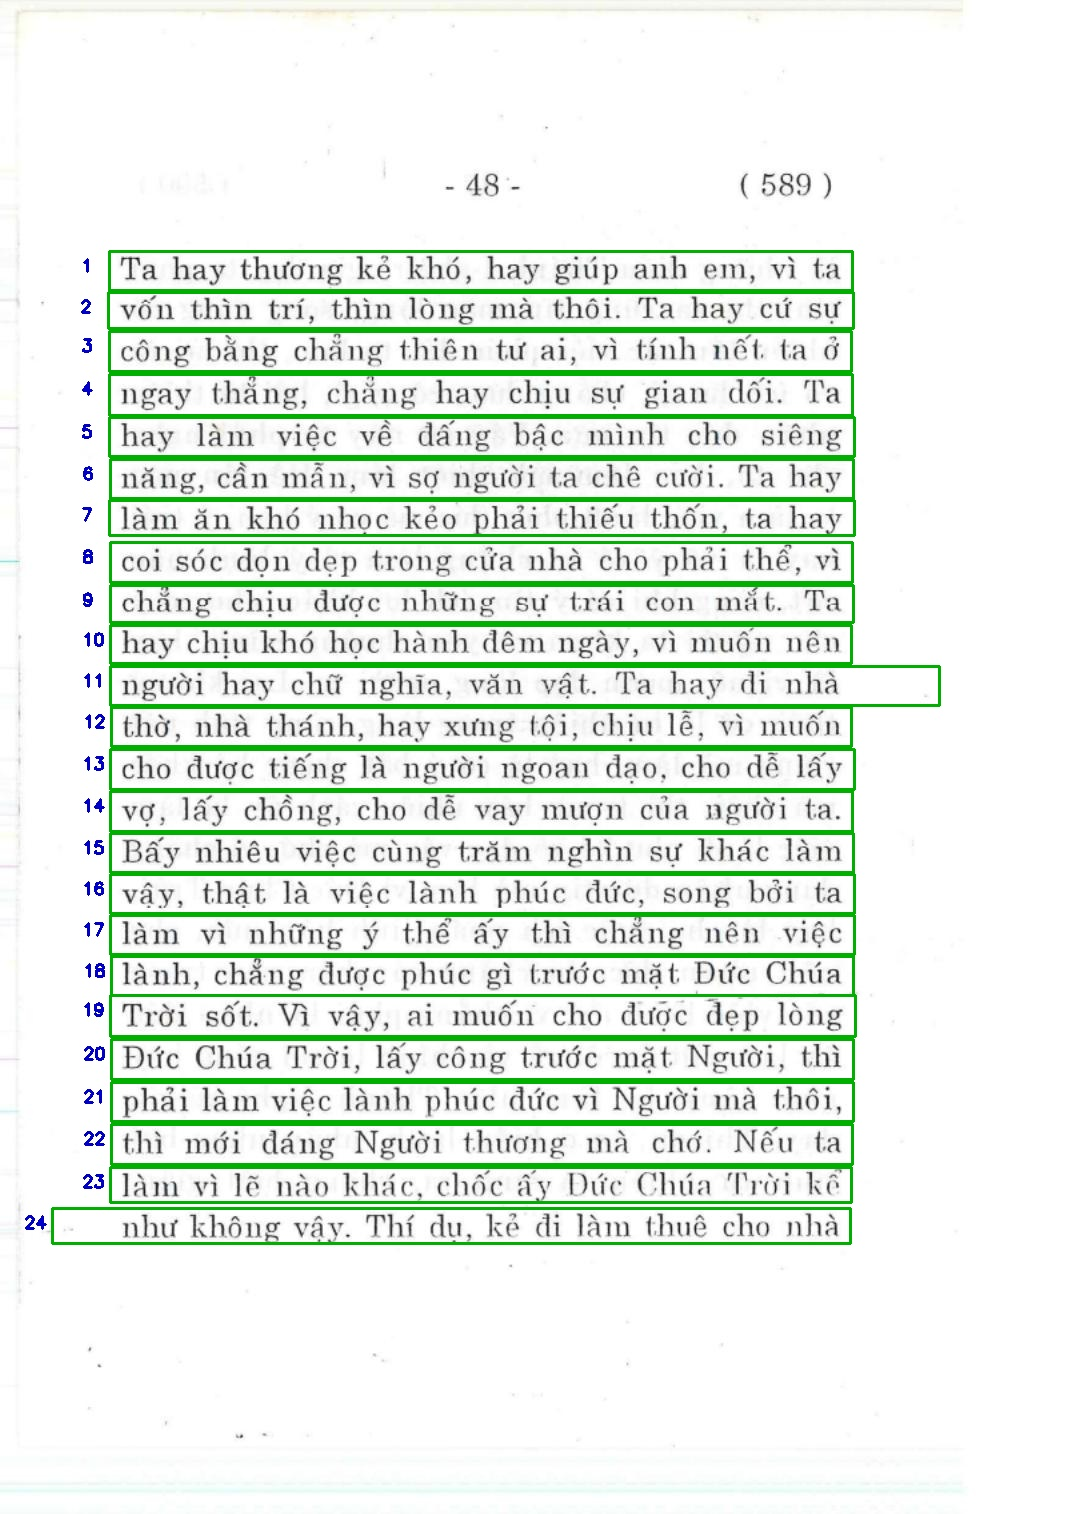
\includegraphics[width=\linewidth, height=0.38\textheight, keepaspectratio]{images/preview_048_boxes.jpg}
        \caption{Trang Quốc ngữ nền sáng tiêu chuẩn (trang in $-48-$)}
    \end{subfigure}\hfill
    \begin{subfigure}[t]{0.48\linewidth}
        \centering
        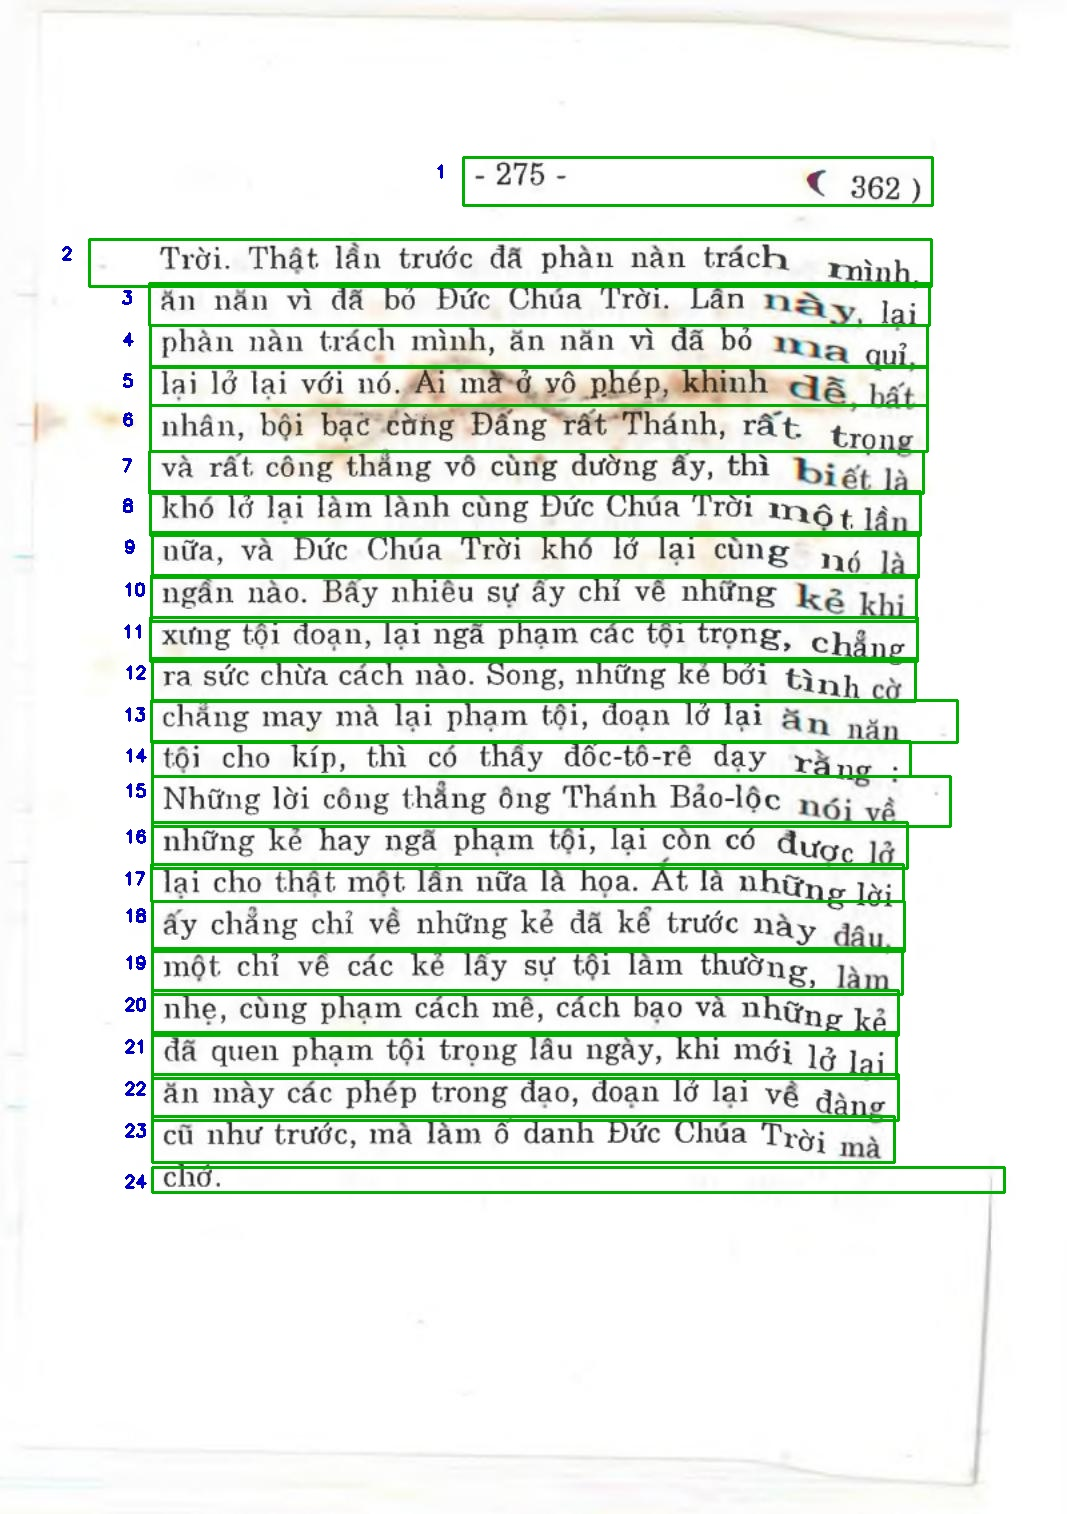
\includegraphics[width=\linewidth, height=0.38\textheight, keepaspectratio]{images/preview_275_boxes.jpg}
        \caption{Trang Quốc ngữ ố vàng nặng (trang in $-275-$)}
    \end{subfigure}
    \caption{Minh họa định vị khung dòng bốn điểm trên ấn bản Quốc ngữ đầu thế kỷ XX cho thấy ranh giới tách biệt giữa dòng tiêu đề số trang và vùng thân trang}
    \label{fig:line_boxes}
\end{figure}

\begin{figure}[H]
    \centering
    \begin{subfigure}[t]{0.48\linewidth}
        \centering
        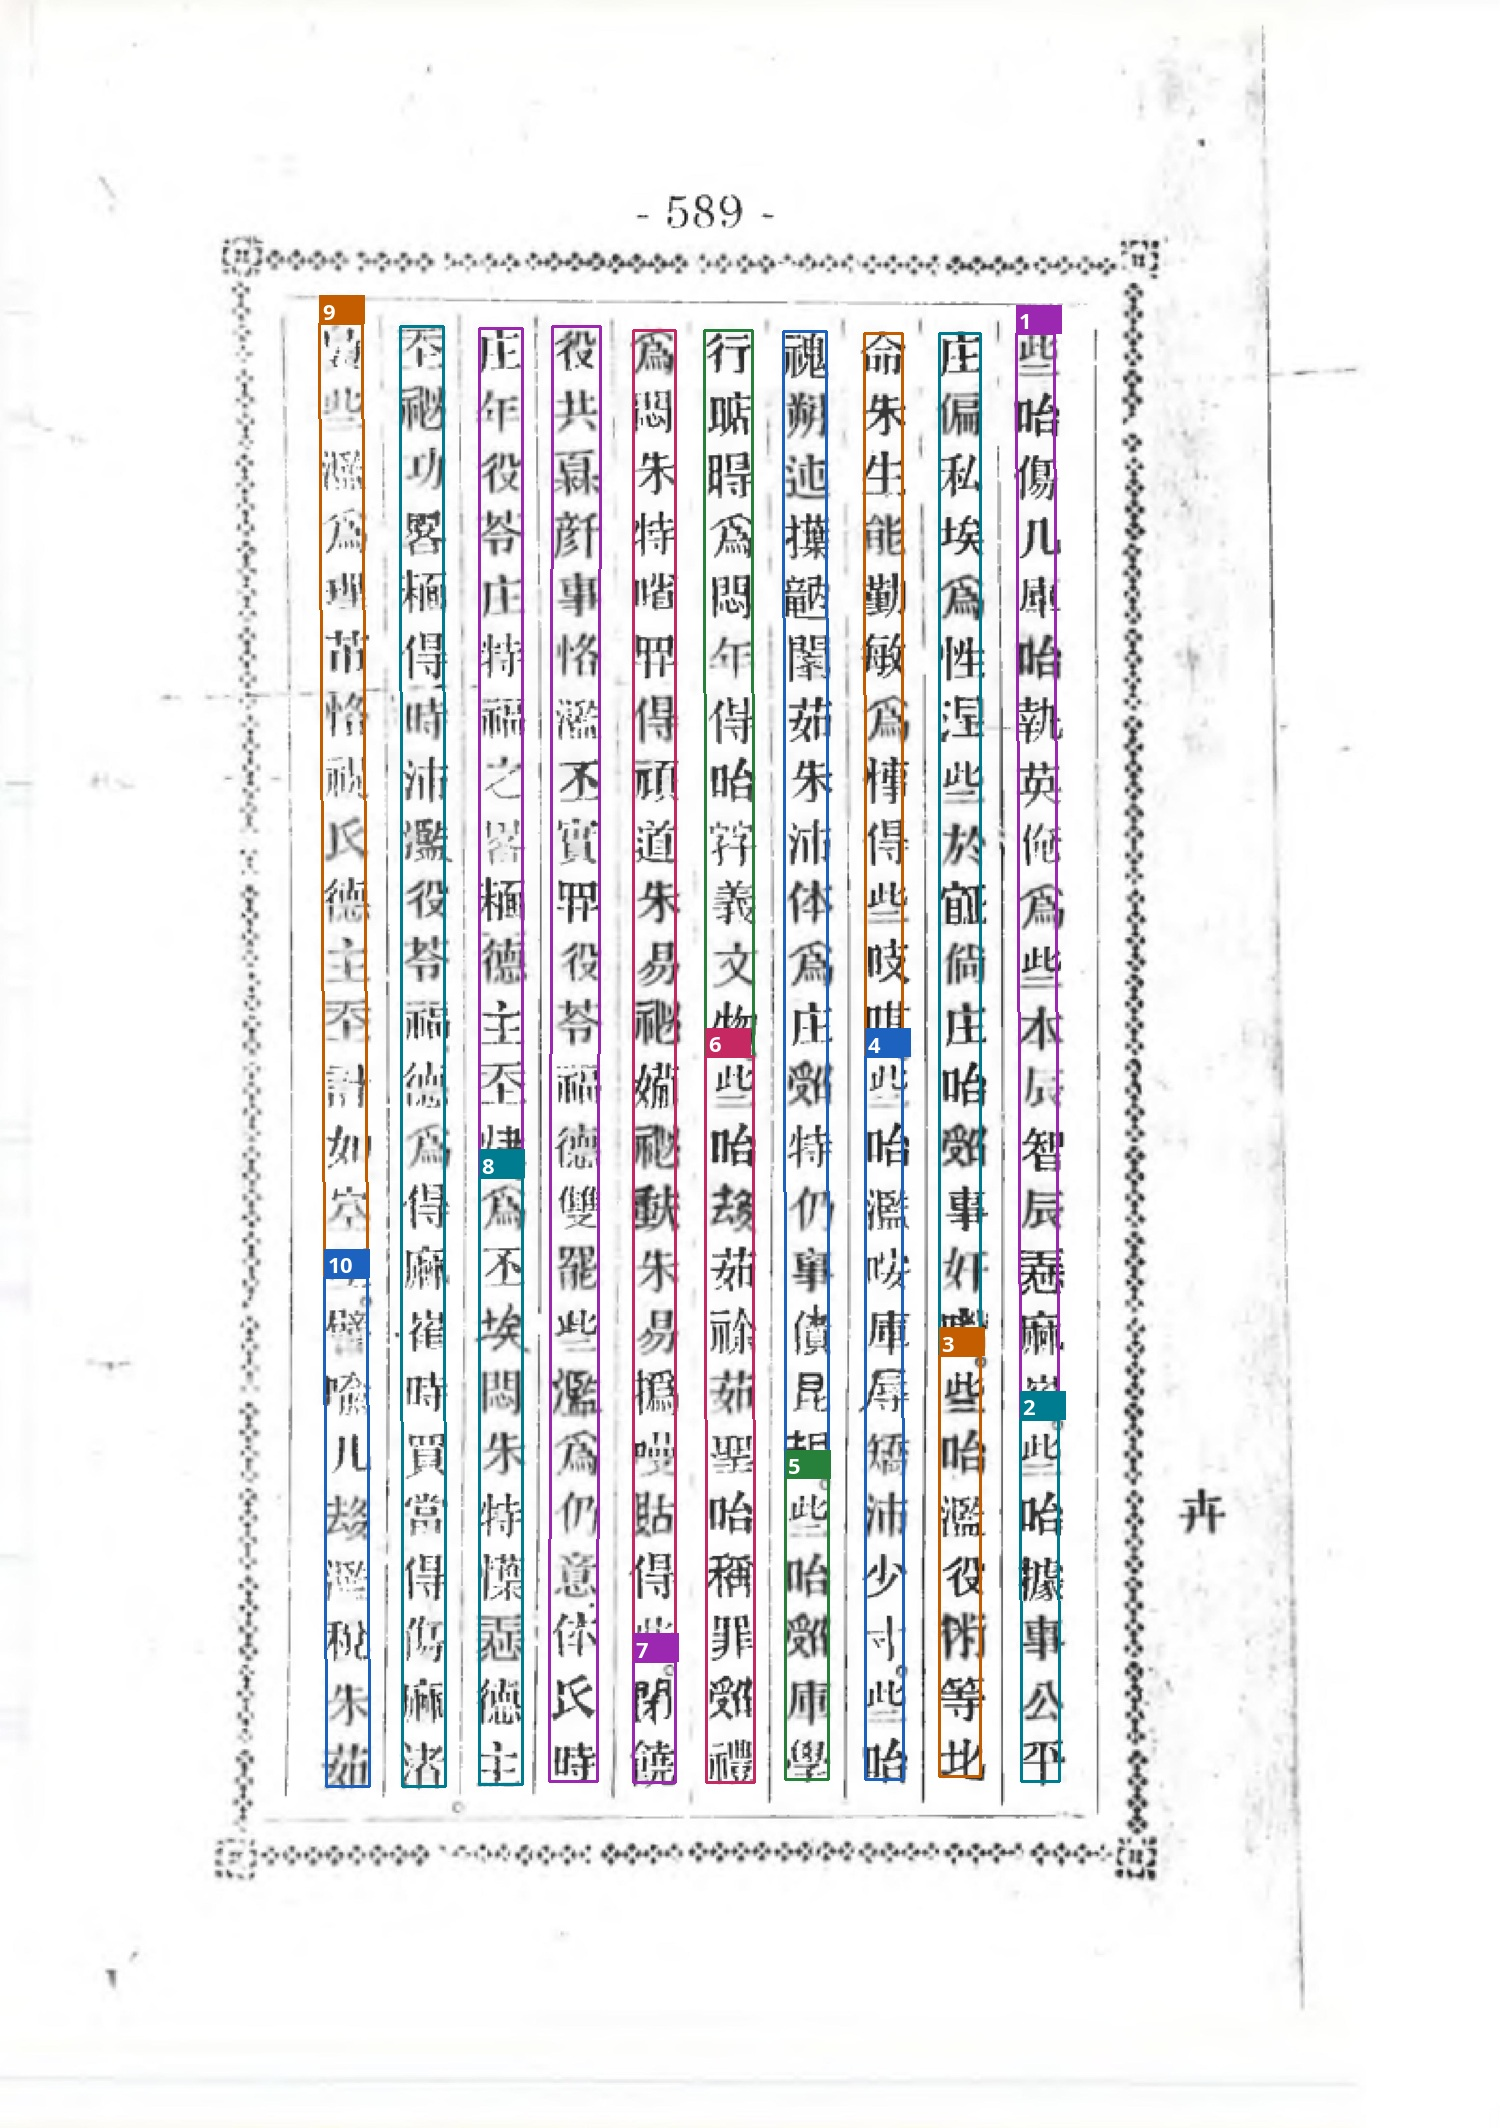
\includegraphics[width=\linewidth, height=0.38\textheight, keepaspectratio]{images/ch_annotated.jpg}
        \caption{Vế Hán Nôm đọc dọc phải sang trái (trang in $-589-$)}
    \end{subfigure}\hfill
    \begin{subfigure}[t]{0.48\linewidth}
        \centering
        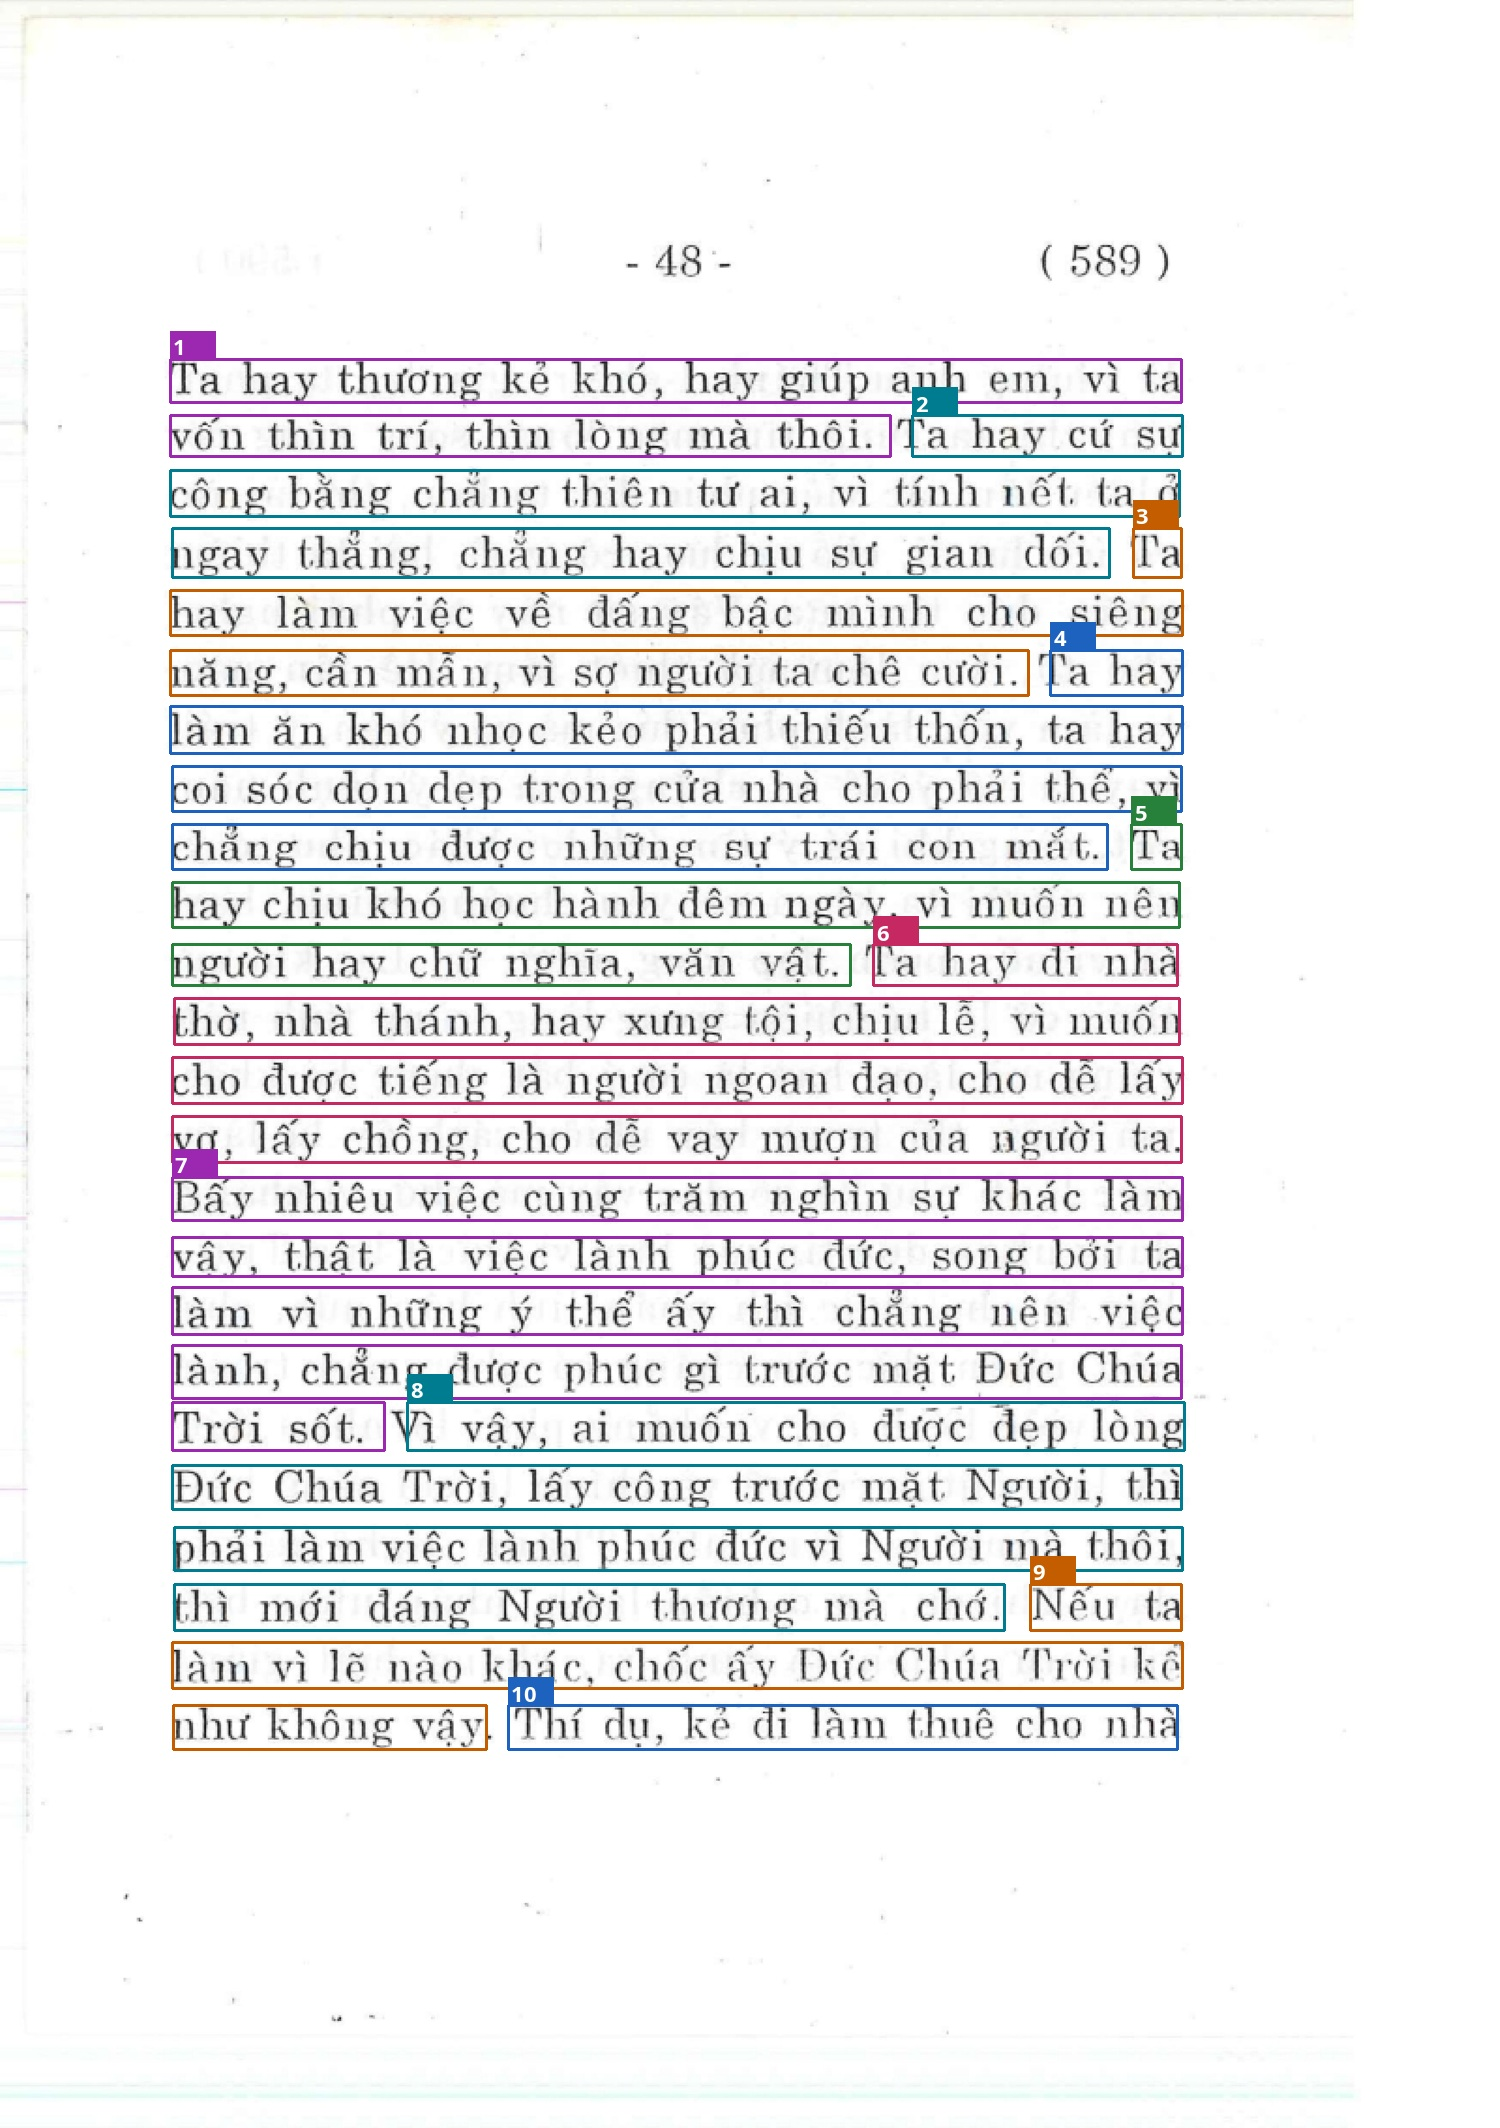
\includegraphics[width=\linewidth, height=0.38\textheight, keepaspectratio]{images/vi_annotated.jpg}
        \caption{Vế Quốc ngữ đọc ngang trái sang phải (trang in $-48-$)}
    \end{subfigure}
    \caption{Minh họa kết quả chiếu ranh giới câu bằng quy hoạch động hai tầng trên cặp trang đối ứng thực tế với $10$ câu song ngữ được khoanh vùng đồng bộ mã màu giữa hai hệ chữ viết}
    \label{fig:parallel_align}
\end{figure}
